\section{Introduction}
\label{sec:Introduction}
This paper seeks to discuss different methods to automate the measurement of cartilage thickness in the human knee using MRI scans. The methods are based on previous work by Wolfgang Wirth and Felix Eckstein. \cite{wirth2008technique}
\par\noindent
All computational methods make use of segmented MRI scans of the human knee, from the OAI dataset, and are written in Python. More precisely, there were two distinct sets of segmentations used: One set of manually segmented images, containing 507 samples, and one set of automatically segmented images, containing 24,783 samples. The set of automatic segmentations contained samples from the entire OAI dataset, i.e. over all time periods. Manual segmentations are stored as MHD and automatic segmentations as NIFTI files, respectively, which can be read and converted into Numpy arrays using the SimpleITK library. These arrays map each point in the three-dimensional space of the scan to an integer encoding of the segmentation, meaning for example points belonging to the femoral cartilage are assigned a value of 3. This makes isolating and extracting the cartilage volumes straightforward. Four different methods have been developed to determine mean cartilage thickness, plus other statistical measures. Thickness was measured for different subregions of the cartilage plate, which were determined as referenced in \cite{wirth2008technique}. For a more detailed description of the procedure, refer to appendix \ref{sec:Subregions}. 

\section{Mean cartilage thickness using meshes}
\label{sec:Meshes}
This is a three-dimensional approach using meshes and normal vectors to determine the mean thickness of a cartilage volume. The main idea is building an upper and a lower mesh, and calculating the average distance between the two, by ray tracing along the normal vectors of the lower mesh against the upper mesh. Other methods, like a K-D-tree nearest neighbour search, are also possible, but have not been implemented. The mesh building is relatively trivial for the tibial cartilage due to its physical shape. Some formal definitions are necessary:
\begin{theorem}[Point Cloud]
	Each cartilage is represented by a set of vectors $V$. The vectors $v \in V$ are defined as a triplet $(x, y, z)$, with $x$, $y$ and $z$ denoting a unique position in the three-dimensional Euclidean space, such that $\forall u, v \in V: u \neq v$.
\end{theorem}
\begin{theorem}[Mesh]
	A mesh is a Delaunay-triangulated surface $DT(P) = (V, E, N)$ of a point cloud $P$, such that no point $p \in P$ lies inside the circumcircle of any triangle in $DT(P)$. \cite{enwiki:delaunay} $DT(P)$ consists of a set of vertices $V$, a set of edges $E$ and a set of surface normals $N$, where $V \equiv P$, $\lvert V \rvert = \lvert N \rvert$.
\end{theorem}
The point cloud representation of the tibial cartilage is obtained by filtering the aforementioned array representation of the MRI scan for the integer encoding specific to the tibial cartilage. The vectors forming the upper and lower surface of the cartilage, respectively, are defined as follows:
\begin{algorithm}
	\caption{Point Cloud Representation of the Cartilage}
	\label{algo:pointcloud}
	\begin{algorithmic}[1]
		\Procedure{CartilageExtraction}{A,C}
		\State $A \gets \text{image array}$
		\State $C \gets \text{color code} \in \{3,4\}$
		\State $P \gets \{\emptyset\}$
		\ForEach{$(x,y,z) \in A$}
			\If{$A[(x,y,z)] = C$}
				\State $P \gets P \cup (x,y,z)$
				\State
			\EndIf
		\EndFor
		\Return $P$
		\EndProcedure
	\end{algorithmic}
\end{algorithm}
Let $P$ be the point cloud representing the tibial cartilage. Furthermore, let $P_{u}$, $P_{l}$ be the point clouds representing the upper and lower surface of the tibial cartilage. Let $f: \mathbb{N} \times \mathbb{N} \rightarrow \mathbb{N}; X \times Y \mapsto \mathbf{Z}$ be a function where $X$ and $Y$ are scalars representing x and y values in the three-dimensional Euclidean space, and $\mathbf{Z}$ be the vector of all $z$ values in the Euclidean space for the position $(x,y)$. Then $P_{u}$ and $P_{l}$ are defined as:
\newline
\begin{equation}
	P_{u} := \{\:(x,y,z)_i \in P \:|\: z = max(f(x,y))\:\}
\end{equation}
\begin{equation}
	P_{l} := \{\:(x,y,z)_i \in P \:|\: z = min(f(x,y))\:\}
\end{equation}
\newline
This essentially means grouping $P$ by $x$ and $y$ coordinates and for each unique coordinate pair $(x_i, y_i)$ in the Euclidean space, choosing the vector with the maximum $z$ coordinate for the upper point cloud $P_{u}$, and the vector with the minimum $z$ coordinate for the lower point cloud $P_{l}$. The result is two point clouds consisting of vectors $(x, y, z)$, as seen in figure \ref{fig:tibial_point_cloud} (red points make up the upper cloud, green the lower). These are then converted into polygon meshes making use of the Delaunay triangulation. For the lower surface mesh, its surface normals are calculated. A surface normal vector is defined as the vector perpendicular to the tangent plane of the surface at a point $P$ \cite{enwiki:normal}. Finally, mean cartilage thickness, i.e. the mean distance between the two meshes, is calculated by tracing along the normal vectors of the lower mesh against the upper mesh. To this end, each surface normal is iteratively extended until it hits the upper mesh, and the Euclidean norm of the vector, i.e. its length, and therefore the distance between the two meshes at a specific point, is computed. This is done for all surface normals, and the average, standard deviation of the calculated distances as well as the mean of the minimum (maximum) 1\% of measurements. Due to the orthogonal nature of the normals, these traces can take into account the topography of the cartilage, allowing for more accurate distance measurements than going in the same static direction for every point $p \in P_{l}$. For other methods not making use of surface normals, like the previously mentioned nearest neighbour search, the Delaunay triangulation may be omitted.
\begin{algorithm}
	\caption{Upper and Lower Point Clouds (Tibia)}
	\label{algo:tibialpointclouds}
	\begin{algorithmic}[1]
		\Procedure{PointClouds}{P}
		\State $P_{u} \gets \max_z (P.groupby((x,y)))$
		\State $P_{l} \gets \min_z (P.groupby((x,y)))$
		\State
		\Return $P_{u}, P_{l}$
		\EndProcedure
	\end{algorithmic}
\end{algorithm} 
\begin{algorithm}
	\caption{Mean Cartilage Thickness (Tibia)}
	\label{algo:tibialthickness}
	\begin{algorithmic}[1]
		\Procedure{TibialThickness}{$P_{u}$, $P_{l}$}
		\State $D \gets \{\emptyset\}$
		\State $M_{u} \gets delaunay(P_{u})$
		\State $M_{l} \gets delaunay(P_{l})$
		\State $N_{l} \gets normals(M_{l})$
		\ForEach{$n \in N_{u}$}
			\State $v \gets raytrace(n, M_{u}$)
			\State $d \gets \norm{v}$
			\State $D \gets D \cup d$
		\EndFor
		\State $\overline{D} \gets \frac{\sum_{i = 0} d_{i} \in D}{\lvert D \rvert}$
		\State
		\Return $\overline{D}$
		\EndProcedure
	\end{algorithmic}
\end{algorithm}
\begin{figure}[]
	\centering
	\includegraphics[width=\linewidth]{./figures/2560px-Normal_vectors_on_a_curved_surface.svg}
	\caption{A curved surface showing the unit normal vectors (blue arrows) to the surface. \cite{surfacenormals}}
	\label{fig:surfacenormals}
\end{figure}
\begin{figure}[]
	\centering
	\includegraphics[width=\linewidth]{./figures/femur_yz}
	\caption{Coronal view on the femoral cartilage. The red bar illustrates the problem of extracting the inner and outer outline by $z$ value: In the posterior part of the cartilage, points that, in reality belong to the outer outline, are assigned to the inner outline, and vice versa.}
	\label{fig:coronal_femur}
\end{figure}
\begin{figure}[]
	\centering
	\includegraphics[width=\linewidth]{./figures/posterior_femur_yz}
	\caption{Coronal view on the posterior part of the femoral cartilage. The part has been rotated to allow outline extraction by z value.}
	\label{fig:coronal_posterior_femur}
\end{figure}
\par
Mesh building for the femoral cartilage is not as trivial. Due to its convex shape, obtaining the upper and lower point clouds $P_{u}$ and $P_{l}$ can not be achieved by simply always taking the maximum (minimum) $z$ value for each coordinate pair $(x,y)$. For an illustration of the problem, refer to figure \ref{fig:coronal_femur}. Using the same approach as for the tibia results in point clouds where some areas are left bare, as illustrated in figure \ref{fig:femoral_point_cloud}. This issue can be circumvented by splitting the cartilage into parts, and rotating problematic sections in such a way that it is once again possible to choose points according to the $z$ coordinate, as illustrated in figure. For a detailed description of how this splitting is achieved, refer to appendix \ref{sec:Splitting}. For each part, the outlines are extracted and meshes are calculated analogous to the tibia, and the meshes' surface normals are used to calculate mean thickness for each part of the femoral cartilage.
\begin{figure}[]
	\centering
	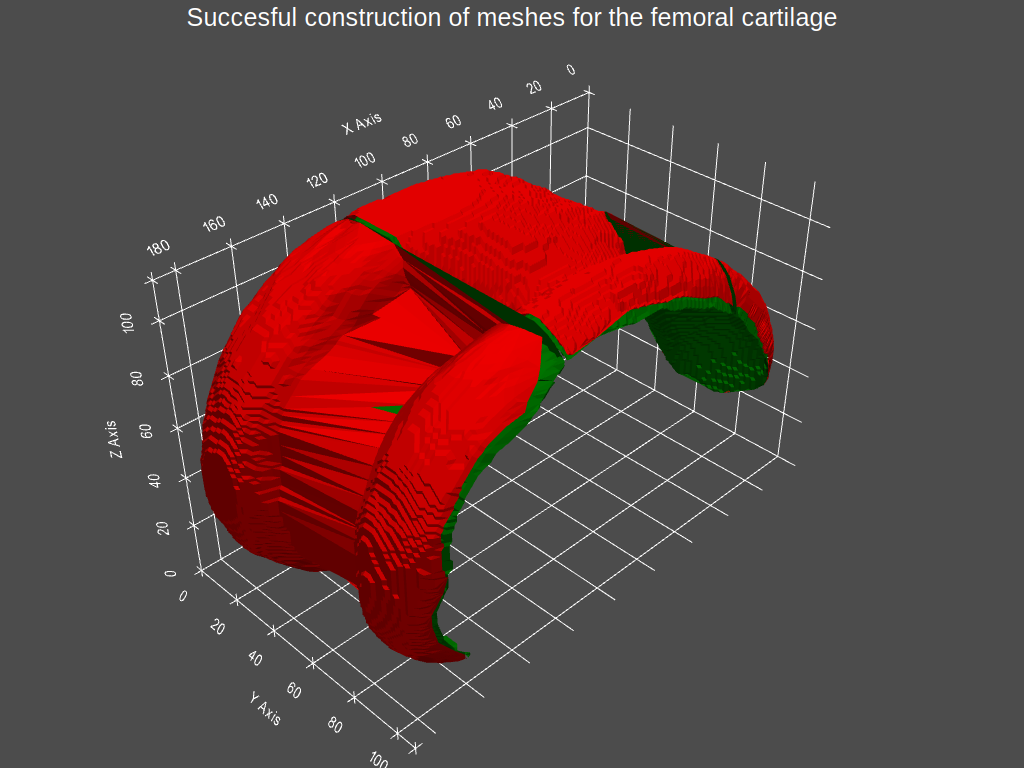
\includegraphics[width=\linewidth]{./figures/femoral_meshes}
	\caption{Triangulated surface meshes for the femoral cartilage.}
	\label{fig:femoral_meshes}
\end{figure}
\begin{figure}[]
	\centering
	\includegraphics[width=\linewidth]{./figures/tibial_meshes}
	\caption{Triangulated surface meshes for the tibial cartilage.}
	\label{fig:tibial_meshes}
\end{figure}
\section{Mean cartilage thickness using ray tracing from a central point}
\label{sec:Raytracing}
This is a three-dimensional approach using ray tracing along normal vectors to determine the mean thickness of a cartilage volume. This is another proposed solution to the previously discussed issue with the convex shape of the femoral cartilage. Instead of fitting meshes to the cartilage, a sphere is constructed around a central point above or below the cartilage A sphere is defined as follows:
\begin{theorem}[sphere]
	A sphere $S = (c, r, V, E, N)$ is a surface mesh, where $c$ is the central point with coordinates $(x,y,z)$, $r$ is the radius, $V$ is a set of vertices, $E$ is a set of edges and $N$ is a set of surface normals, such that $\lvert V \rvert = \lvert N \rvert$.
\end{theorem}
Let $P$ be the point cloud representing a cartilage $C$. Then 
\begin{flalign*}
	c &= (x,y,z);&&\\
	c_x &= \min_{x} P + (\max_{x} P - \min_{x} P) \div 4&&\\
	c_y &= \min_{y} P + (\max_{y} P - \min_{y} P) \div 2&&\\
	c_z &= \min_{z} P + (\max_{z} P - \min_{z} P) \div 2&&\\
\end{flalign*}
for the central weight-bearing zones,
\begin{flalign*}
	c_x &= \min_{x} P + (\max_{x} P - \min_{x} P) \div 4&&\\
	c_y &= \min_{y} P + (\max_{y} P - \min_{y} P) \div 2&&\\
	c_z &= \min_{z} P + (\max_{z} P - \min_{z} P) \div 2&&\\
\end{flalign*}
for the medial and lateral posterior femoral cartilage,
\begin{flalign*}
	c_x &= \min_{x} P + ((\max_{x} P - \min_{x} P) \div 4) \cdot 3&&\\
	c_y &= \min_{y} P + (\max_{y} P - \min_{y} P) \div 2&&\\
	c_z &= \min_{z} P + (\max_{z} P - \min_{z} P) \div 4&&\\
\end{flalign*}
for the medial and lateral anterior femoral cartilage, and
\begin{flalign*}
	c_x &= \min_{x} P + (\max_{x} P - \min_{x} P) \div 2&&\\
	c_y &= \min_{y} P + (\max_{y} P - \min_{y} P) \div 2&&\\
	c_z &= \max_{z} P \:\cdot\: 1.25&&\\
\end{flalign*}
for the lateral and medial tibial cartilage.
\bigskip
\par\noindent
$\lvert V \rvert$ corresponds to the resolution of the sphere, which is a tuple $(\theta, \phi)$, where $\theta$ is the number of vertices in the horizontal (longitude) direction, and $\phi$ the number of vertices in the vertical (latitude) direction. $\theta$ should be equal to $\phi$ in order to obtain a real sphere, as opposed to an ellipsoid; in our case, $\theta = \phi = 60$, and therefore $lvert V \rvert = 60 + 59 \cdot 58 = 3,482$.
Given a point cloud $P$ and a sphere $S = (c, r, V, E, N)$, the thickness of the corresponding cartilage can be calculated with the following procedure:
Each surface normal $n \in N$ is iteratively extended until it hits a point $p \in P$, or a maximum number of iterations is reached, in which case the normal is discarded. Once a point is hit, its position is saved as $p_1$, and $n$ is further extended until no more points are hit. For every iteration of this further extension, the hit point in that iteration is saved as $p_2$. At the end of the iteration, the Euclidean distance between the first hit $p_1$ and the last hit $p_2$ is calculated.
This approach is one of the more computationally expensive ones, as for one, generally more than half of the surface normals will never make a hit, and tracing along these is a wasted effort, although this may be remedied somewhat by checking whether the search space, i.e. the point cloud, lies in the direction of the vector a priori. The other major reason is that the nature of ray tracing is inherently expensive.
\begin{algorithm}
	\caption{Ray Tracing from a Sphere}
	\label{algo:raytracing}
	\begin{algorithmic}[1]
		\Procedure{RayTracing}{$P, S$}
		\State $D \gets \{\emptyset\}$
		\ForEach{$n \in N$}
			\Repeat
				\State $n \gets n \cdot 2$
				\If{$n \in P$}
					\State $p_1 \gets n$
					\State \textit{break}
				\EndIf
			\Until{iterations $> 100$}
			\Repeat
				\State $n \gets n \cdot 2$
				\If{$n \notin P$}
					\State \textit{break}
				\EndIf
				\State $p_2 \gets n$
			\Until{iterations $> 100$}
			\State $dist \gets d(p_1, p_2)$
			\State $D \gets D \cup dist$
			\State
		\EndFor 
		\State $\overline{D} \gets \frac{\sum_{i = 0} d_{i} \in D}{\lvert D \rvert}$
		\State
		\Return $\overline{D}$
		\EndProcedure
	\end{algorithmic}
\end{algorithm}
\begin{figure}[]
	\centering
	\includegraphics[width=\linewidth]{./figures/sphere_placement_femur}
	\caption{Exemplary placement of a sphere for the lateral posterior femoral cartilage.}
	\label{fig:femoral_sphere}
\end{figure}
\begin{figure}[]
	\centering
	\includegraphics[width=\linewidth]{./figures/sphere_placement_tibia}
	\caption{Exemplary placement of a sphere for the lateral tibial cartilage.}
	\label{fig:tibial_sphere}
\end{figure}
\section{Mean cartilage thickness using two-dimensional function fitting}
\label{sec:Function_fitting}
\subsection{Determine thickness via function normals}
\label{sec:Normals}
This approach is settled in the two-dimensional rather than the three-dimensional Euclidean space. Instead of considering the MRI scan as a whole, and thus the entire cartilage, the idea here is to look at slices instead. A cartilage is divided into layers, and a polynomial function through the centre is obtained by a least-square fit. A number of normals can then be calculated, making use of the derivative of the function. Since the normal of a function $f$ at a point $x$ is perpendicular to the tangent of $f$ at $x$, the thickness of the cartilage at that point can accurately be determined by finding the outermost intersection points of the normal with the cartilage in either direction, and computing the Euclidean distance between the two intersection points. Do this for every slice and average over the individual measurements to obtain the mean thickness of the cartilage. The advantage of this approach is that the polynomial functions are generally easier to fit than the triangulated meshes discussed earlier, bar for some edge cases (e.g. the outermost slices of the cartilage, where data points can be very sparse and thus, getting a good fit is difficult if not impossible). On the other hand, some sections may be omitted from calculations, as can be seen in figure \ref{fig:normals}.
\begin{algorithm}
	\caption{Normals of a Polynomial Fit}
	\label{algo:normals}
	\begin{algorithmic}[1]
		\Procedure{FunctionNormals}{P}
		\State $D \gets \{\emptyset\}$
		\State $L \gets \textit{convertIntoLayers(P)}$
		\ForEach{$layer \: l \in L$}
			\State $f \gets \textit{polyfit(l)}$
			\State $\nabla f \gets \textit{derivative(f)}$
			\State $N \gets \textit{normals(f)}$
			\ForEach{$n \in N$}
				\State $m \gets \textit{slope(n)}$
				\State $p_1 \gets \textit{lastIntersection(n, m)}$
				\State $p_2 \gets \textit{lastIntersection(n, -m)}$
				\State $dist \gets d(p_1, p_2)$
				\State $D \gets D \cup dist$
				\State
			\EndFor
		\EndFor
		\State $\overline{D} \gets \frac{\sum_{i = 0} d_{i} \in D}{\lvert D \rvert}$
		\State
		\Return $\overline{D}$
		\EndProcedure
	\end{algorithmic}
\end{algorithm}
\begin{figure}[]
	\centering
	\includegraphics[width=\linewidth]{./figures/normals}
	\caption{Normals along a two-dimensional least squares fit}
	\label{fig:normals}
\end{figure} 

\subsection{Determine thickness via integration/function values}
\label{sec:Integration}
This approach is also settled in the two-dimensional Euclidean space, the difference to the previous being that there are two polynomial functions instead of one, which don't go through the middle of the cartilage but rather are fit along its outlines, as illustrated in figure \ref{fig:integration}. The distance between the functions, i.e. the thickness of the cartilage, can then easily be calculated, for example by integrating both functions and taking the difference ($\int f(x) dx - \int g(x) dx$), or calculating the difference between the function values for every $x$ value ($[\sum_{x_i = 0}^{\max_{x}} f(x_i) - g(x_i)] \cdot \frac{1}{\max_{x}}$). Since no normals and therefore no intersection points have to be calculated, this approach is the computationally least expensive. The downside is that it can not take the topography of the cartilage into account, resulting in less accurate measurements especially for the anterior and posterior parts of the femoral cartilage. This can be somewhat remedied by making use of splines, i.e. splitting the cartilage into multiple parts in a similar fashion to the procedure used for the earlier discussed mesh building.
\par
As previously mentioned, one issue with both of these approaches is that the function fitting may not work well for certain shapes, especially for layers where the number of data points is very sparse. Although most of the layers are going to have no more than two inflection points (layers of the femoral cartilage can generally be approximated by a second-order polynom, while the layers of the tibial cartilage tend to follow a third-order form), some edge cases, e.g. the outermost layers, might return a poor fit, or no fit at all. This could possibly be remedied by choosing a higher degree for the polynomial fit, but doing so may in turn lead to undesirable effects (overfitting, Runge's phenomenon, etc.).
\begin{figure}[]
	\centering
	\includegraphics[width=\linewidth]{./figures/integration}
	\caption{Two functions fit over the outlines of a tibial cartilage slice exposure}
	\label{fig:integration}
\end{figure}